
\let\negmedspace\undefined
\let\negthickspace\undefined
\documentclass[journal]{IEEEtran}
\usepackage[a5paper, margin=10mm, onecolumn]{geometry}
%\usepackage{lmodern} % Ensure lmodern is loaded for pdflatex
\usepackage{tfrupee} % Include tfrupee package
\setlength{\headheight}{1cm} % Set the height of the header box
\setlength{\headsep}{0mm}     % Set the distance between the header box and the top of the text
\usepackage{gvv-book}
\usepackage{gvv}
\usepackage{cite}
\usepackage{amsmath,amssymb,amsfonts,amsthm}
\usepackage{algorithmic}
\usepackage{graphicx}
\usepackage{textcomp}
\usepackage{xcolor}
\usepackage{txfonts}
\usepackage{listings}
\usepackage{enumitem}
\usepackage{mathtools}
\usepackage{gensymb}
\usepackage{comment}
\usepackage[breaklinks=true]{hyperref}
\usepackage{tkz-euclide} 
\usepackage{listings}
% \usepackage{gvv}                                        
\def\inputGnumericTable{}                                 
\usepackage[latin1]{inputenc}                                
\usepackage{color}                                            
\usepackage{array}                                            
\usepackage{longtable}                                       
\usepackage{calc}                                             
\usepackage{multirow}                                         
\usepackage{hhline}                                           
\usepackage{ifthen}                                           
\usepackage{lscape}
\renewcommand{\thefigure}{\theenumi}
\renewcommand{\thetable}{\theenumi}
\setlength{\intextsep}{10pt} % Space between text and floats
\numberwithin{equation}{enumi}
\numberwithin{figure}{enumi}
\renewcommand{\thetable}{\theenumi}
\begin{document}
\bibliographystyle{IEEEtran}
\title{12.6.5.12}
\author{EE24BTECH11041 - Mohit}
% \maketitle
% \newpage
% \bigskip
{\let\newpage\relax\maketitle}
\begin{enumerate}
\item Find the maximum and minimum values of $x + \sin{2x}$ on $\brak{ 0,2\pi }$\\
\textbf{Solution}:-
\begin{enumerate}
\item Theoritical Solution:-
\begin{align}
y = x + \sin{2x}\\
\end{align}
Differentiating on both side,
\begin{align}
\frac{dy}{dx} = 1 + 2\cos{2x}
\end{align}
Putting $\frac{dy}{dx} =  0$
\begin{align}
1 + 2\cos{2x} = 0\\
\cos{2x} = -\frac{1}{2}\\
x = \frac{1}{2}\cos{\brak{-\frac{1}{2}}}
\end{align}
The value of $x$ we get in interval in $\brak{0,2\pi}$,
\begin{align}
 x = \frac{\pi}{3},\frac{2\pi}{3},\frac{4\pi}{3},\frac{5\pi}{3}
\end{align}
Again differentaiting , Equation 1.6 ,
\begin{align}
\frac{d^2y}{dx^2} = -4\sin{2x}
\end{align} 
Putting the value of $x$ in Equation 1.8 ,We will get $-4\sin{2x}$ negative for $x= \frac{\pi}{3},\frac{4\pi}{3}$ and positive for $x = \frac{2\pi}{3},\frac{5\pi}
{3}$\\
Hence, we will get maxima for $x= \frac{\pi}{3},\frac{4\pi}{3}$ and minima for $x = \frac{2\pi}{3},\frac{5\pi}{3}$\\
Value of Function when maxima occur is is 1.91 and 5.05 and when maxima occur is 1.23 and 4.36 . \\
But we have to consider initial and final values of Function in interval $\brak{0,2\pi}$ .\\
Value of function at $x=0$ is 0 and at $x=2\pi$ is 6.29
Therefore, minimum value of function is 0 and maximum value $2\pi$.
\end{enumerate}
\textbf{CODING LOGIC:-}

Define the function:
    \begin{align}
    f(x) = x + \sin(2x)
    \end{align}

    \textbf{Set parameters for gradient descent and ascent:}
    \begin{enumerate}
        \item Learning rate ($ \eta $) = 0.01
        \item Maximum iterations = 10,000
        \item Tolerance  = $1 \times 10^{-6}$
    \end{enumerate}
    
    \textbf{Initialize starting points}
    \begin{align}
    \text{start\_points} = \text{linspace}(0, 2\pi, 50)
    \end{align}
    A range of 50 equally spaced starting points between $0$ and $2\pi$ is chosen to search for critical points.\\
    
    \textbf{Use C functions for gradient descent and ascent}\\
     And Value of $x$ changes as:-
     \begin{align}
     \eta = 0.01
     \end{align}
     \begin{align}
     x_{n+1} = x_{n} + \eta\frac{dy}{dx_n} \text{ ,when gradient is positive}\\
     x_{n+1} = x_{n} - \eta\frac{dy}{dx_n} \text{ ,when gradient is negative}
     \end{align}
     Change in value of x depends on gradient ,\\
     \textbf{Find critical points - }
     For each starting point, we use both gradient descent and ascent to find the corresponding critical points:

     \textbf{Classify critical points:}
     \begin{enumerate}
        \item Minima are identified by checking the slope:
        \begin{align}
        f(x + 1 \times 10^{-3}) - f(x - 1 \times 10^{-3}) > 0
        \end{align}
        \item Maxima are identified by :-
        \begin{align}
        f(x + 1 \times 10^{-3}) - f(x - 1 \times 10^{-3}) < 0
        \end{align}
    \end{enumerate}
    
\end{enumerate}
\begin{figure}[h!]
   \centering
   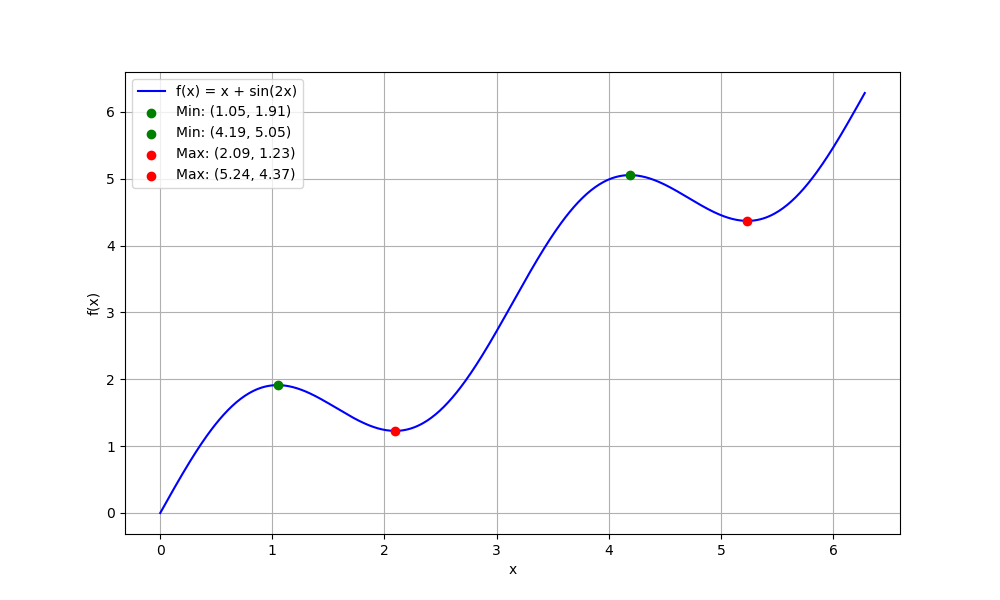
\includegraphics[width=0.7\linewidth]{figs/Figure_1.png}
\end{figure}

\end{document}
